\documentclass{article}

\usepackage{fancyhdr}
\usepackage{extramarks}
\usepackage{amsmath}
\usepackage{amsthm}
\usepackage{amsfonts}
\usepackage{tikz}
\usepackage[plain]{algorithm}
\usepackage{algpseudocode}
\usepackage{enumerate}
\usepackage{tikz}
\usepackage{listings}

\usetikzlibrary{automata,positioning}

%
% Basic Document Settings
%  

\topmargin=-0.45in
\evensidemargin=0in
\oddsidemargin=0in
\textwidth=6.5in
\textheight=9.0in
\headsep=0.25in

\linespread{1.1}

\pagestyle{fancy}
\lhead{\hmwkAuthorName}
\chead{\hmwkClass : \hmwkTitle}
\rhead{\firstxmark}
\lfoot{\lastxmark}
\cfoot{\thepage}

\renewcommand\headrulewidth{0.4pt}
\renewcommand\footrulewidth{0.4pt}

\setlength\parindent{0pt}

%
% Create Problem Sections
%

\newcommand{\enterProblemHeader}[1]{
    \nobreak\extramarks{}{Problem \arabic{#1} continued on next page\ldots}\nobreak{}
    \nobreak\extramarks{Problem \arabic{#1} (continued)}{Problem \arabic{#1} continued on next page\ldots}\nobreak{}
}

\newcommand{\exitProblemHeader}[1]{
    \nobreak\extramarks{Problem \arabic{#1} (continued)}{Problem \arabic{#1} continued on next page\ldots}\nobreak{}
    \stepcounter{#1}
    \nobreak\extramarks{Problem \arabic{#1}}{}\nobreak{}
}

\newcommand*\circled[1]{\tikz[baseline=(char.base)]{
		\node[shape=circle,draw,inner sep=2pt] (char) {#1};}}


\setcounter{secnumdepth}{0}
\newcounter{partCounter}
\newcounter{homeworkProblemCounter}
\setcounter{homeworkProblemCounter}{1}
\nobreak\extramarks{Problem \arabic{homeworkProblemCounter}}{}\nobreak{}

%
% Homework Problem Environment
%
% This environment takes an optional argument. When given, it will adjust the
% problem counter. This is useful for when the problems given for your
% assignment aren't sequential. See the last 3 problems of this template for an
% example.
%

\newenvironment{homeworkProblem}[1][-1]{
    \ifnum#1>0
        \setcounter{homeworkProblemCounter}{#1}
    \fi
    \section{Problem \arabic{homeworkProblemCounter}}
    \setcounter{partCounter}{1}
    \enterProblemHeader{homeworkProblemCounter}
}{
    \exitProblemHeader{homeworkProblemCounter}
}

%
% Homework Details
%   - Title
%   - Class
%   - Due date
%   - Name
%   - Student ID

\newcommand{\hmwkTitle}{Homework\ \#11}
\newcommand{\hmwkClass}{Probability \& Statistics for EECS}
\newcommand{\hmwkDueDate}{April 30, 2023}
\newcommand{\hmwkAuthorName}{Zhou Shouchen}
\newcommand{\hmwkAuthorID}{2021533042}


%
% Title Page
%

\title{
    \vspace{2in}
    \textmd{\textbf{\hmwkClass:\\  \hmwkTitle}}\\
    \normalsize\vspace{0.1in}\small{Due\ on\ \hmwkDueDate\ at 23:59}\\
	\vspace{4in}
}

\author{
	Name: \textbf{\hmwkAuthorName} \\
	Student ID: \hmwkAuthorID}
\date{}

\renewcommand{\part}[1]{\textbf{\large Part \Alph{partCounter}}\stepcounter{partCounter}\\}

%
% Various Helper Commands
%

% Useful for algorithms
\newcommand{\alg}[1]{\textsc{\bfseries \footnotesize #1}}
% For derivatives
\newcommand{\deriv}[1]{\frac{\mathrm{d}}{\mathrm{d}x} (#1)}
% For partial derivatives
\newcommand{\pderiv}[2]{\frac{\partial}{\partial #1} (#2)}
% Integral dx
\newcommand{\dx}{\mathrm{d}x}
% Alias for the Solution section header
\newcommand{\solution}{\textbf{\large Solution}}
% Probability commands: Expectation, Variance, Covariance, Bias
\newcommand{\E}{\mathrm{E}}
\newcommand{\Var}{\mathrm{Var}}
\newcommand{\Cov}{\mathrm{Cov}}
\newcommand{\Bias}{\mathrm{Bias}}

\begin{document}

\maketitle

\pagebreak

\begin{homeworkProblem}[1]
(a) $(X,Y,X+Y)$ is MVN.\\

Let $Z = t_1X+t_2Y+t_3(X+Y)$, then $Z = (t_1+t_3)X+(t_2+t_3)Y$.\\
Since $X,Y$ are i.i.d, and $X,Y\sim N(0,1)$, from what we have learn, the sum of indepedent normal distributions is still a normal distribution.\\
And since $Z=(t_1+t_3)X+(t_2+t_3)Y$, so $Z$ is the linear combination of two indepedent normal distribution, so $Z$ is a still a Normal.\\
So $\forall t_1,t_2,t_3$, $Z$ is a normal. From the defination of MVN, we can say that $(X,Y,X+Y)$ is MVN.\\

So above all, $(X,Y,X+Y)$ is MVN.\\

(b) $(X,Y,SX+SY)$ is not MVN.\\
Let $Z = t_1X+t_2Y+t_3(SX+SY)$, take $t_1=t_2=t_3=1$, then $Z=(1+S)X+(1+S)Y$.\\
So $P(Z=0)=P((1+S)(X+Y)=0)=P(S=-1)+P(X=-Y)-P(S=-1,X=-Y)$.\\
Since $X,Y$ are indepedent continous random variables, so $P(X=-Y)=0$.\\
And since $S$ is the random signal, so $P(S=-1)=\dfrac{1}{2}$.\\
And since $S$ is indepedent with $(X,Y)$, so $P(S=-1,X=-Y)=P(S=-1)P(X=-Y)=0$.\\
So $P(Z=0)=\dfrac{1}{2}$.\\
And this means that when $t_1=t_2=t_3$, $Z$ is a discrete random variable, not even a continous variable, so it must not be Normal.\\

So above all, $(X,Y,SX+SY)$ is not MVN.\\
  
(c) $(SX,SY)$ is MVN.\\
Let $Z = t_1(SX)+t_2(SY)$, then $Z = S(t_1X+t_2Y)$.\\
Let $W=t_1X+t_2Y$, from the property of MVN, we know that $W$ is the linear combination of two i.i.d. Normal, so $W$ is alse Normal.\\
Also, $X,Y\sim N(0,1)$, so $W\sim N(0,t_1^2+t_2^2)$, which means that $W$ is symmetric about $x=0$.\\
Since $Z=SW$, $S$ is the random signal, so $P(S=1)=P(S=-1)=\dfrac{1}{2}$. With LOTP, we can get that\\
$P(Z\leq z)=P(SW\leq z|S=1)P(S=1)+P(SW\leq z|S=-1)P(S=-1)=\dfrac{1}{2}P(W\leq z)+\dfrac{1}{2}P(-W\leq z)$.\\
From the symmetric property of $W$, we can get that $P(-W\leq z)=P(W\geq -z)=P(W\leq z)$.\\
So $P(Z\leq z)=P(W\leq z)$.\\
So $Z$ and $W$ have the same CDF, so $Z$ is also Normal.\\

So above all, $(SX,SY)$ is MVN.\\

\end{homeworkProblem}

\newpage

\begin{homeworkProblem}[2]
(1) using the properties of MVN.\\
Since X,Y are i.i.d. and $X,Y\sim N(0,1)$, so $T=X+Y$ and $W=X-Y$ are combinations of two i.i.d. Normal, so $T,W$ are Normal.\\
Let $Z=t_1T+t_2W$, then $Z=(t_1+t_2)X+(t_1-t_2)Y$.\\
So $Z\sim N(0,(t_1+t_2)^2+(t_1-t_2)^2)=N(0,2(t_1^2+t_2^2))$.\\
So $\forall t_1,t_2$, $Z$ is a Normal.\\
From the defination of MVN, we can say that $(T,W)$ is MVN.\\
i.e. $(T,W)$ is Bivariate Normal.\\
And their covariance is that\\
$\Cov(T,W)=\Cov(X+Y,X-Y)=\Cov(X,X)-\Cov(X,Y)+\Cov(Y,X)-\Cov(Y,Y)=Var(X)-Var(Y)$.\\
Since $X,Y\sim N(0,1)$, so $Var(X)=Var(Y)=1$.\\
So $\Cov(T,W)=0$.\\
i.e. $Corr(T,W)=0$.\\
Since $(T,W)$ is Bivariate Normal, and $Corr(T,W)=0$, so $T,W$ are indepedent.\\
So above all, $T,W$ are indepedent.\\

(2) using the change of variable.\\
Since X,Y are i.i.d. and $X,Y\sim N(0,1)$, so $f_X(x)=\dfrac{1}{\sqrt{2\pi}}e^{-\frac{1}{2}x^2},f_Y(y)=\dfrac{1}{\sqrt{2\pi}}e^{-\frac{1}{2}y^2}$.\\
And since $T=X+Y,W=X-Y$, so $X=\dfrac{T+W}{2},Y=\dfrac{T-W}{2}$.\\
So the Jacobian determinant is that $J=\big|\dfrac{\partial(x,y)}{\partial(t,w)}\big|=\begin{vmatrix}
\frac{\partial x}{\partial t} & \frac{\partial x}{\partial w}\\
\frac{\partial y}{\partial t} & \frac{\partial y}{\partial w}
\end{vmatrix}=\begin{vmatrix}
\frac{1}{2} & \frac{1}{2}\\
\frac{1}{2} & -\frac{1}{2}
\end{vmatrix}=-\dfrac{1}{2}$.\\
So with the property of transformation, we can get that\\
$f_{T,W}(t,w)=f_{X,Y}(x,y)|J|=\dfrac{1}{\sqrt{2\pi}}e^{-\frac{1}{2}x^2}\cdot \dfrac{1}{\sqrt{2\pi}}e^{-\frac{1}{2}y^2}\cdot\dfrac{1}{2}=\dfrac{1}{4\pi}e^{-\frac{1}{4}(t^2+w^2)}$\\
$=(\dfrac{1}{\sqrt{2\pi}\sqrt{2}}e^{-\frac{1}{2\cdot (\sqrt{2})^2}t^2})\cdot (\dfrac{1}{\sqrt{2\pi}\sqrt{2}}e^{-\frac{1}{2\cdot (\sqrt{2})^2}w^2})$.\\
So the joint PDF can be write into two parts' multiplication.\\
i.e. $f_{T,W}(t,w)=g(t)h(w)$, where $g(t)=(\dfrac{1}{\sqrt{2\pi}\sqrt{2}}e^{-\frac{1}{2\cdot (\sqrt{2})^2}t^2}),h(w)=(\dfrac{1}{\sqrt{2\pi}\sqrt{2}}e^{-\frac{1}{2\cdot (\sqrt{2})^2}w^2})$.\\
So we can let $f_T(t)=g(t)=\dfrac{1}{2\sqrt{\pi}}e^{-\frac{1}{4}t^2}$, $f_W(w)=h(w)=\dfrac{1}{2\sqrt{\pi}}e^{-\frac{1}{4}w^2}$.\\
From the PDF of $T,W$, we can get that: $T,W\sim N(0,2)$.\\

Check:\\
Since the domain of $T,W$ have no couple, and $T,W\sim N(0,2)$, which means that we get the valid PDF.\\
So we can say that $T,W$ are indepedent.\\

So above all, $T,W$ are indepedent.\\

\end{homeworkProblem}

\newpage

\begin{homeworkProblem}[3]
From the discription, we can get that $X=R\cdot cos\Theta, Y=R\cdot sin\Theta$.\\
So the Jacobian determinant is that $J=\big|\dfrac{\partial(x,y)}{\partial(r,\theta)}\big|=\begin{vmatrix}
\frac{\partial x}{\partial r} & \frac{\partial x}{\partial \theta}\\
\frac{\partial y}{\partial r} & \frac{\partial y}{\partial \theta}
\end{vmatrix}=\begin{vmatrix}
cos\theta & -r\cdot sin\theta\\
sin\theta & r\cdot cos\theta
\end{vmatrix}=r\cdot cos^2\theta+r\cdot sin^2\theta=r$.\\
Since $X,Y$ are i.i.d. $N(0,1)$, so $f_X(x)=\dfrac{1}{\sqrt{2\pi}}e^{-\frac{1}{2}x^2},f_Y(y)=\dfrac{1}{\sqrt{2\pi}}e^{-\frac{1}{2}y^2}$.\\
So with the property of transformation, we can get that\\
$f_{R,\Theta}(r,\theta)=f_{X,Y}(x,y)|J|=\dfrac{1}{\sqrt{2\pi}}e^{-\frac{1}{2}x^2}\cdot \dfrac{1}{\sqrt{2\pi}}e^{-\frac{1}{2}y^2}\cdot r=\dfrac{1}{2\pi}e^{-\frac{1}{2}r^2}\cdot r$.\\
So the joint PDF can be write into two parts' multiplication.\\
i.e. $f_{R,\Theta}(r,\theta)=g(r)h(\theta)$, where $g(r)=re^{-\frac{1}{2}r^2},h(\theta)=\dfrac{1}{2\pi}$.\\
So we can let $f_R(r)=g(r)=r\cdot e^{-\frac{1}{2}r^2}$, $f_{\Theta}(\theta)=h(\theta)=\dfrac{1}{2\pi}$.\\

Check:\\
The domain of $T,W$ have no couple.
And from the decription, we can get that the domain of $R,\Theta$ is that $r\in[0,+\infty)$ and $\theta\in [0,2\pi]$.\\
So $\int_{0}^{2\pi}f_{\Theta}(\theta)=\int_{0}^{2\pi}\dfrac{1}{2\pi}=1$.\\
So $f_{\Theta}(\theta)$ is a valid PDF, from the theorem we have learned, we could get that $f_R(r)$ is also a valid PDF.\\
So we can say that $R,\Theta$ are indepedent.\\

So above all, the joint distribution of $R,\Theta$ is that $f_{R,\Theta}(r,\theta)=\dfrac{1}{2\pi}r\cdot e^{-\frac{1}{2}r^2}$.\\
And $R,\Theta$ are indepedent.\\

\end{homeworkProblem}

\newpage

\begin{homeworkProblem}[4]
(a) Since $X,Y$ are i.i.d. $Expo(\lambda)$, so $f_X(x)=\lambda e^{-\lambda x},x>0$,\\
and $f_Y(y)=\lambda e^{-\lambda y},y>0$.\\
And since $T=X+Y,W=\dfrac{X}{Y}$, so $X=\dfrac{WT}{W+1},Y=\dfrac{T}{W+1}$.\\
So we can get that the Jacobian determinant is that\\
$J=\big|\dfrac{\partial(x,y)}{\partial(t,w)}\big|=\begin{vmatrix}
    \frac{\partial x}{\partial t} & \frac{\partial x}{\partial w}\\
    \frac{\partial y}{\partial t} & \frac{\partial y}{\partial w}
\end{vmatrix}=\begin{vmatrix}
    \frac{w}{w+1} & \frac{t}{(w+1)^2}\\
    \frac{1}{w+1} & \frac{-t}{(w+1)^2}
\end{vmatrix}=\dfrac{-t}{(w+1)^2}$.\\
Since $t>0,w>0$, so $|J|=\dfrac{t}{(w+1)^2}$.\\
So with the property of transformation, we can get that\\
$f_{T,W}(t,w)=f_{X,Y}(x,y)|J|=\lambda e^{-\lambda x}\cdot \lambda e^{-\lambda y}\cdot \dfrac{t}{(w+1)^2}=\lambda^2 te^{-\lambda t}\cdot \dfrac{1}{(w+1)^2}$.\\

So the joint PDF can be write into two parts' multiplication.\\
i.e. $f_{T,W}(t,w)=g(t)h(w)$, where $g(t)=\lambda^2 te^{-\lambda t},h(w)=\dfrac{1}{(w+1)^2}$.\\
So we can let $f_T(t)=g(t)=\lambda^2 te^{-\lambda t}$, $f_W(w)=h(w)=\dfrac{1}{(w+1)^2}$.\\

Check:
The domain of $T,W$ have no couple.\\
And from the decription, we can get that the domain of $T$ is that $t\in(0,+\infty)$ and the domain of $W$ is that $w\in (0,+\infty)$.\\
And since $\int_{0}^{+\infty}f_W(w)=\int_{0}^{+\infty}\dfrac{1}{(w+1)^2}dw=-\dfrac{1}{w+1}\big|_{0}^{+\infty}=1$, $f_W(w)$ is strictly increasing in its support, $f_W(w)\geq 0$.\\
So $f_W(w)$ is a valid PDF, from the theorem we have learned, we could get that $f_T(t)$ is also a valid PDF.\\
And $g(t),h(w)$ are the marginal PDFs of $T$ and $W$.\\

So above all, the joint distribution of $T,W$ is that $f_{T,W}(t,w)=\lambda^2 te^{-\lambda t}\cdot \dfrac{1}{(w+1)^2}$.\\
And the marginal PDFs of $T,W$ is that $f_T(t)=\lambda^2 te^{-\lambda t}, t>0$, $f_W(w)=\dfrac{1}{(w+1)^2}, w>0$.\\

(b) Since $X,Y,Z$ are i.i.d $Unif(0,1)$, so $f_X(x)=f_Y(y)=f_Z(z)=1, x,y,z\in[0,1]$
Let $T = Y+Z$. Then $T\in [0,2]$.\\
And since $W=X+Y+Z$, so $W\in [0,3]$.\\

1. Firstly, we can calculate the PDF of $T$ using convolution.\\
When $t\in[0,1]$, $f_T(t)=\int_{0}^{t}f_Y(y)f_Z(t-y)dy=\int_{0}^{t}dy=t$.\\
When $t\in(1,2]$, $f_T(t)=\int_{t-1}^{1}f_Y(y)f_Z(t-y)dy=\int_{t-1}^{1}dy=1-(t-1)=2-t$.\\
Otherwise, $f_T(t)=0$.\\

2. Secondly, we can calculate the PDF of $W$ using convolution, and we can regard $Y+Z$ as a group $T$.\\
When $w\in[0,1]$, $x\in [0,w]$, so $f_W(w)=\int_{0}^{w}f_X(x)f_T(w-x)dx=\int_{0}^{w}(w-x)dx=\dfrac{1}{2}w^2$.\\
When $w\in(1,2]$, $t\in [w-1,w]$, so $f_W(w)=\int_{w-1}^{w}f_T(t)f_X(w-t)dt=\int_{w-1}^{1}tdt+\int_{1}^{w}(2-t)dt=-w^2+3w-\dfrac{3}{2}$.\\
When $w\in(2,3]$, $x\in [w-2,1]$, so $f_W(w)=\int_{w-2}^{1}f_X(x)f_T(w-x)dx=\int_{w-2}^{1}(2-(w-x))dx$\\
$=\int_{w-2}^{1}(2+x-w)dx=\dfrac{1}{2}w^2-3w+\dfrac{9}{2}$.\\

So above all, the PDF of $W$ is that $f_W(w)=\begin{cases}
    \dfrac{1}{2}w^2, & w\in[0,1]\\
    -w^2+3w-\dfrac{3}{2}, & w\in(1,2]\\
    \dfrac{1}{2}w^2-3w+\dfrac{9}{2}, & w\in(2,3]\\
    0, & \text{otherwise}
\end{cases}$.\\

(c) Let $Z=\dfrac{1}{2}Y$, since $Y\sim Expo(\lambda)$, so the CDF of $Y$ is $F_Y(y)=1-e^{-\lambda y}$.\\
So the CDF of $Z$ is $F_Z(z)=P(Z\leq z)=P(\dfrac{1}{2}Y\leq z)=P(Y\leq 2z)=F_Y(2z)=1-e^{-2\lambda z}$.\\
So we can see that $Z\sim Expo(2\lambda)$.\\
i.e. $\dfrac{1}{2}Y\sim Expo(2\lambda)$.\\

(1) using properties of Exponential.\\
From the property that we have learned, the Minimum of independent Expos indicates that:\\
If $X_1,\cdots,X_n$ are indepedent, and $X_i\sim Expo(\lambda_i)$, then $L=min(X_1,\cdots,X_n)\sim Expo(\lambda_1+\cdots+\lambda_n)$.\\

Let $L=min(X,Y)$.\\
Since $X,Y$ are i.i.d. $Expo(\lambda)$, so $L\sim Expo(2\lambda)$.\\
From above, we have proved that $\dfrac{1}{2}Y\sim Expo(2\lambda)$, so $L\sim \dfrac{1}{2}Y$.\\
And since $M=max(X,Y)$, so we can get that $M+L=X+Y$.\\
Since $L\sim \dfrac{1}{2}Y$, so $M\sim X+Y-L=X+Y-\dfrac{1}{2}Y=X+\dfrac{1}{2}Y$.\\
So $M$ has the same distribution as $X+\dfrac{1}{2}Y$.\\

(2) using convolution.\\
We can calculate the CDF of $M$. Since $X,Y$ are i.i.d. $Expo(\lambda)$, so\\
$F_M(m)=P(M\leq m)=P(max(X,Y)\leq m)=P(X\leq m,Y\leq m)$\\
$=P(X\leq m)P(Y\leq m)=F_X(m)F_Y(m)=(1-e^{-\lambda m})^2$.\\
So the PDF of $M$ is $f_M(m)=F_M'(m)=2\lambda e^{-\lambda m}-2\lambda e^{-2\lambda m}$.\\

And we can calculate the PDF of $X+\dfrac{1}{2}Y$ using convolution.\\
Let $Z=\dfrac{1}{2}Y$, in the above, we have proved that $Z\sim Expo(2\lambda)$, so for $T=X+Z$, we can get that\\
$f_T(t)=\int_{0}^{t}f_X(x)f_Z(t-x)dx=\int_{0}^{t}\lambda e^{-\lambda x}\cdot 2\lambda e^{-2\lambda (t-x)}dx=2\lambda^2 e^{-2\lambda t}\int_{0}^{t}e^{\lambda x}dx$\\
$=2\lambda^2 e^{-2\lambda t}\cdot \dfrac{1}{\lambda}(e^{\lambda t}-1)=2\lambda e^{-\lambda t}(1-e^{-\lambda t})=2\lambda e^{-\lambda t}-2\lambda e^{-2\lambda t}$.\\

So we can see that $M$ and $Z=X+\dfrac{1}{2}Y$ have the same PDF.\\
So $M$ and $X+\dfrac{1}{2}Y$ have the same distribution.\\

\end{homeworkProblem}

\newpage

\begin{homeworkProblem}[5]
(a) $U\sim Unif(0,2\pi)$, so $f_U(u)=\dfrac{1}{2\pi},u\in [0,2\pi]$.\\
So we can easily sample on $U$.\\

$T\sim Expo(1)$, so $f_T(t)=e^{-t}, t\in (0,+\infty)$.\\
To sample on $T$, we can use the Universality of Uniform as what we have done in Homework8.\\
i.e. From what we have learned, the Exponential distribution has CDF $F(x) = 1 - e^{-x}, \forall x > 0$\\
And its PDF is $f(x) = F'(x) = e^{-x}$\\
Let $ y = F(x) = 1 - e^{-x}, \forall x > 0$, then $e^{-x}=1-y$\\
i.e. $-x = ln(1-y)$, and since $x>0$, so $x = -ln(1-y) $\\
So the inverse funciton of its CDF is $ F^{-1}(x) = -ln(1-x) $\\
Let $U_1\sim Unif(0,1)$
And let $X = F^{-1}(U_1)$, then $X$ is an r.v. with CDF $F$.\\
i.e. we have sample a distribution $X$ with PDF $f(x) = e^{-x}$.\\
So after getting $X$, it is the same as sampling on $T$.\\

Let $X=\sqrt{2T}cos(U), Y=\sqrt{2T}sin(U)$.\\
From Box-Muller method, we can get that $X,Y$ are i.i.d. $N(0,1)$.\\
And we can take the histogram of $X$ as a normal distribution.\\
We can also generate the theoretical PDF by $f_X(x)=\dfrac{1}{\sqrt{2\pi}}e^{-\frac{1}{2}x^2}$.\\
And we can plot them in the same plot, the plot is as followed.\\
\begin{figure}[htbp]
    \centering
    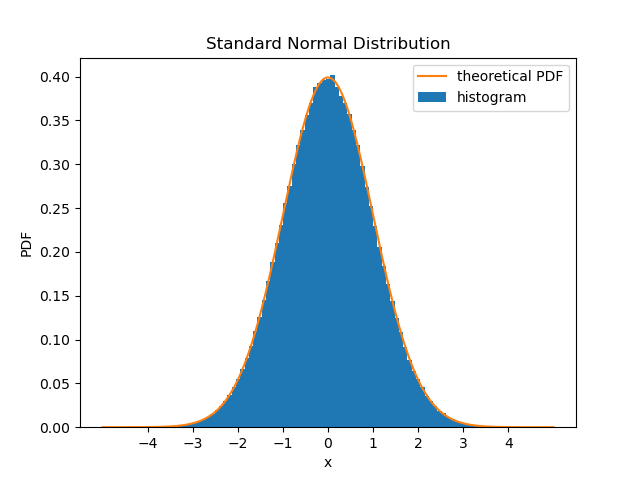
\includegraphics[width=0.9\textwidth]{../result/normal.png}
    \caption{Histogram and theoretical PDF of $X$}
\end{figure}

(c) Let $(Z,W)$ be the standard Bivariate Normal distribution, and take their correlation coefficient to be $\rho$.\\
$X,Y$ are i.i.d. $N(0,1)$, which can be sampled from (a).\\
Let $Z=X, W=\rho X+\sqrt{1-\rho^2}Y$.\\
Then we can get that $Z,W$ are all $N(0,1)$.\\
Also theri correlation coefficient is $\rho$.\\
Which can be easily proved:\\
$Corr(Z,W)=\dfrac{Cov(Z,W)}{\sqrt{Var(Z)Var(W)}}$\\
$=Cov(Z,W)=Cov(X,\rho X+\sqrt{1-\rho^2}Y)=Cov(X,\rho X)+Cov(X,\sqrt{1-\rho^2}Y)=\rho$.\\

To get $Z,W$'s joint PDF, we can use transformation.\\
We have get that $Z=X,W=\rho X+\sqrt{1-\rho^2}Y$.\\
So $X=Z, Y=\dfrac{W-\rho Z}{\sqrt{1-\rho^2}}$.\\
So the Jacobian determinant is $\dfrac{\partial(x,y)}{\partial(z,w)}=\dfrac{1}{\sqrt{1-\rho^2}}>0$.\\
So $f_{Z,W}(z,w)=f_{X,Y}(x,y)\cdot \big|\dfrac{\partial(x,y)}{\partial(z,w)}\big|=f_X(x)f_Y(y)\cdot \dfrac{1}{\sqrt{1-\rho^2}}$.\\
We can respectively take $\rho=0,0.3,0.5,0.7,0.9$.\\
After sampling with the method above, we can plot their figures, and with each figure, we can get their corresponding contours plotting below them.\\
From up to down, for each line, we take $\rho=0,0.3,0.5,0.7,0.9$.\\
And for each line, from left to right, it is the plot of $Z,W$'s joint PDF, sampled scatter plot, and their contour plot.\\

\begin{figure}[htbp]
    \centering
    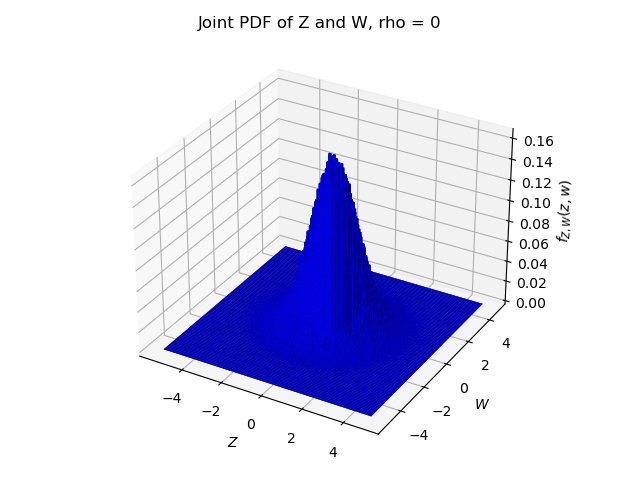
\includegraphics[width=0.3\textwidth,height=0.3\textwidth]{../result/pdf0.png}
    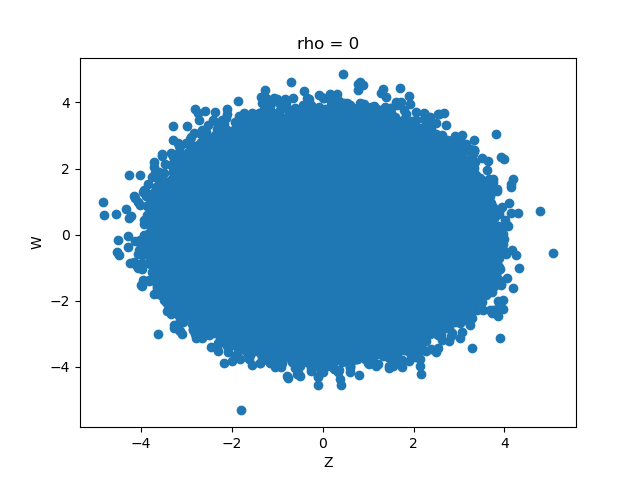
\includegraphics[width=0.3\textwidth,height=0.3\textwidth]{../result/rho0.png}
    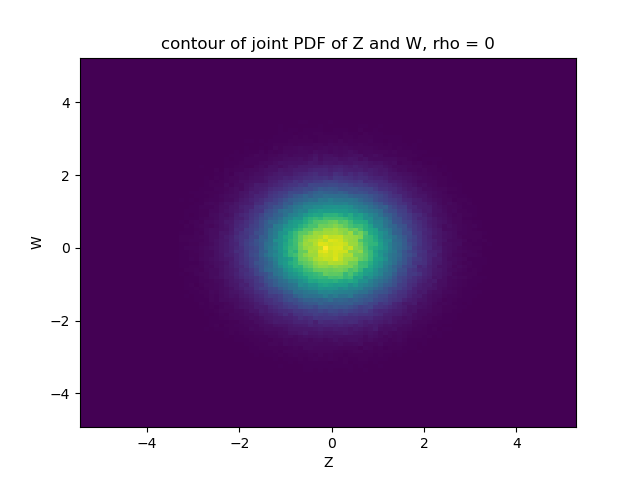
\includegraphics[width=0.3\textwidth,height=0.3\textwidth]{../result/contour0.png}

    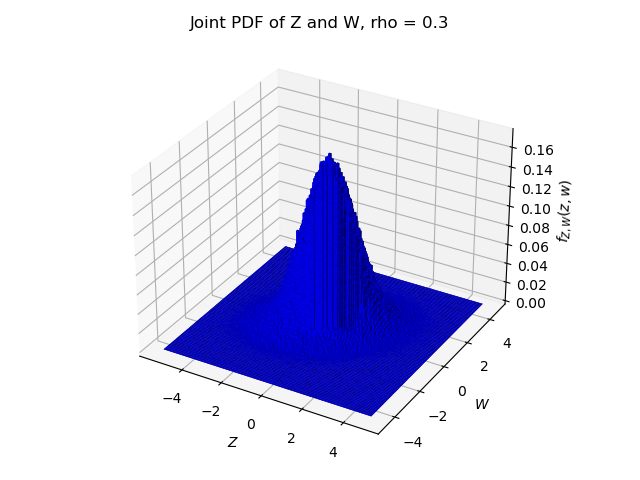
\includegraphics[width=0.3\textwidth,height=0.3\textwidth]{../result/pdf0.3.png}
    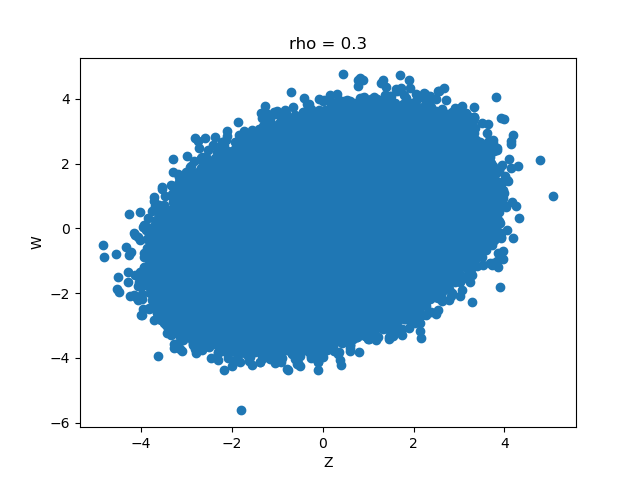
\includegraphics[width=0.3\textwidth,height=0.3\textwidth]{../result/rho0.3.png}
    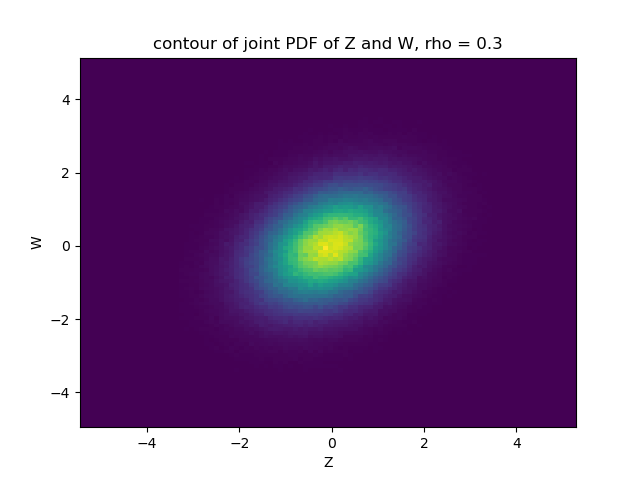
\includegraphics[width=0.3\textwidth,height=0.3\textwidth]{../result/contour0.3.png}

    \caption{Bivariate Noamal distribution with correlation $\rho$ and their contours}
\end{figure}
    
\begin{figure}[htbp]
    \centering
    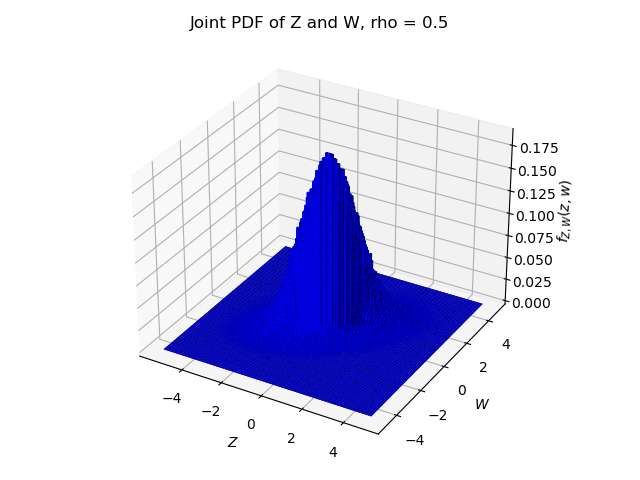
\includegraphics[width=0.3\textwidth,height=0.3\textwidth]{../result/pdf0.5.png}
    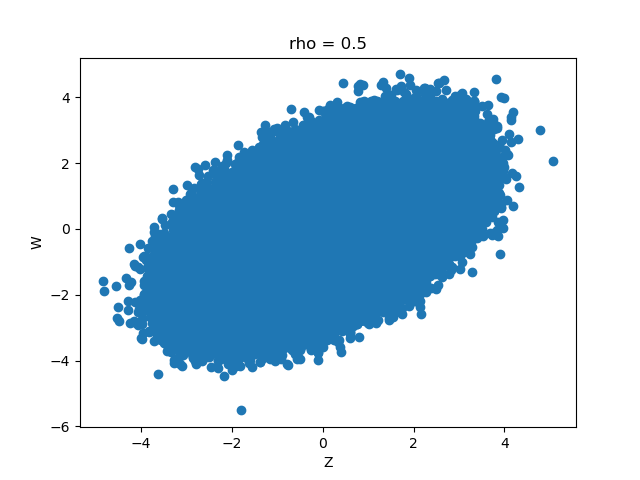
\includegraphics[width=0.3\textwidth,height=0.3\textwidth]{../result/rho0.5.png}
    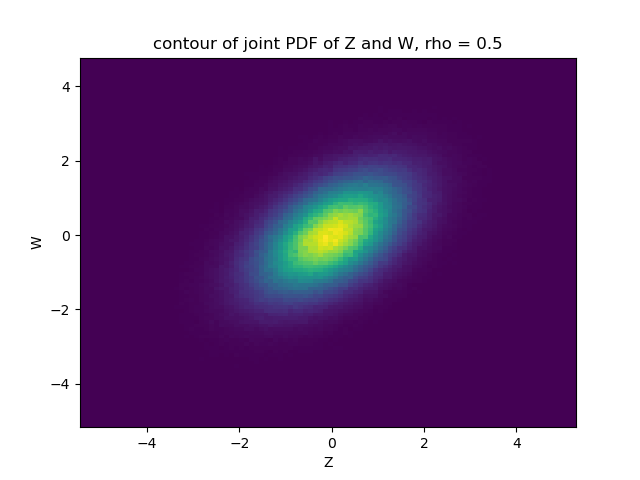
\includegraphics[width=0.3\textwidth,height=0.3\textwidth]{../result/contour0.5.png}

    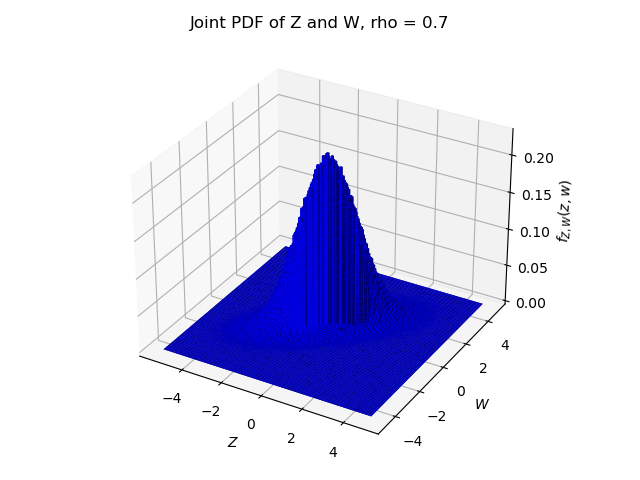
\includegraphics[width=0.3\textwidth,height=0.3\textwidth]{../result/pdf0.7.png}
    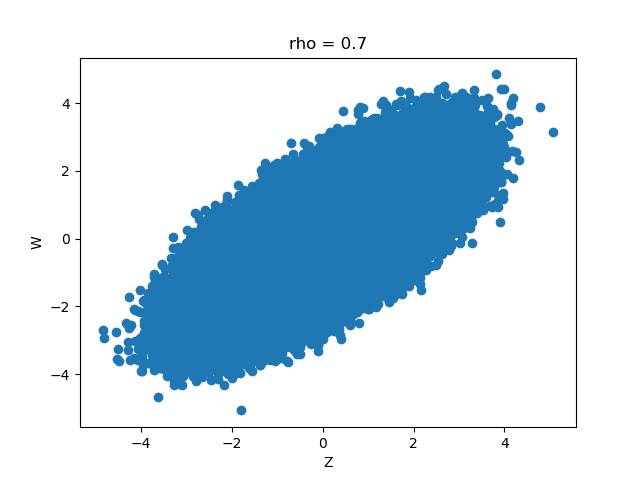
\includegraphics[width=0.3\textwidth,height=0.3\textwidth]{../result/rho0.7.png}
    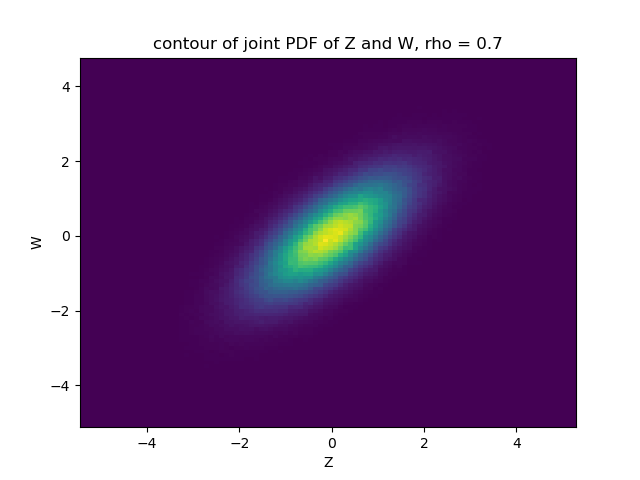
\includegraphics[width=0.3\textwidth,height=0.3\textwidth]{../result/contour0.7.png}

    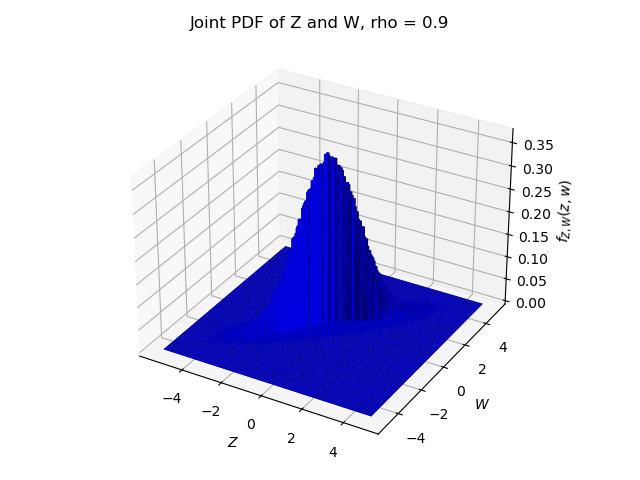
\includegraphics[width=0.3\textwidth,height=0.3\textwidth]{../result/pdf0.9.png}
    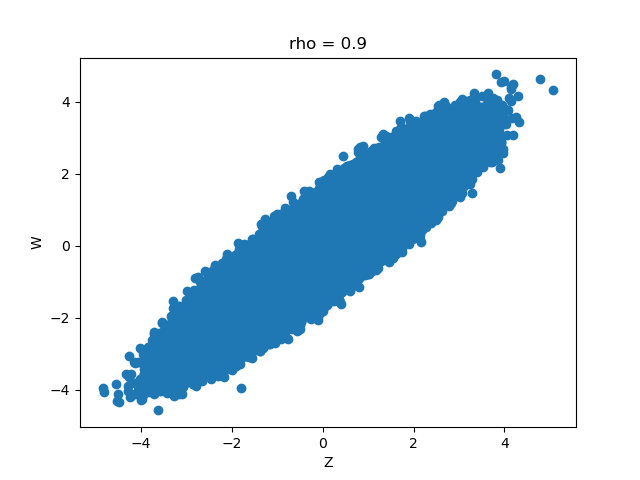
\includegraphics[width=0.3\textwidth,height=0.3\textwidth]{../result/rho0.9.png}
    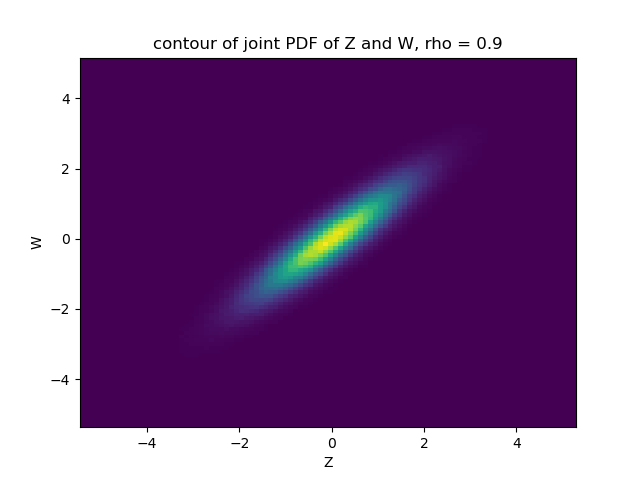
\includegraphics[width=0.3\textwidth,height=0.3\textwidth]{../result/contour0.9.png}

    \caption{Bivariate Noamal distribution with correlation $\rho$ and their contours}
\end{figure}

\begin{lstlisting}[title=appendix(code), frame=shadowbox]
import numpy as np
import matplotlib.pyplot as plt

# Normal distribution
def normal_PDF(x, mu, sigma): # the PDF of the normal distribution
    return 1 / (np.sqrt(2 * np.pi) * sigma) * np.exp(-(x - mu)**2 / (2 * sigma**2))

# Exponential Distribution
def exponential_PDF(x): # the PDF of the exponential distribution
    return np.exp(-x)

def exponential_inverse(x): # the inverse of the exponential distribution
    return -np.log(1 - x)

def inverse_transform_sampling(sample_size): # inverse transform sampling
    u = np.random.uniform(0, 1, sample_size) # uniform random numbers
    return exponential_inverse(u)

sample_size = 1000000

expo = inverse_transform_sampling(sample_size) # sample points using inverse transform sampling
u = np.random.uniform(0, 2 * np.pi, sample_size) # uniform random numbers
X = np.sqrt(2 * expo) * np.cos(u) # sample points using Box-Muller method
Y = np.sqrt(2 * expo) * np.sin(u) # sample points using Box-Muller method

plt.hist(X, bins = 100, density = True)

# plot the standard normal's pdf
x = np.linspace(-5, 5, 1000) # sample points for plotting pdf
pdf = normal_PDF(x, 0, 1) # pdf values at sample points
plt.plot(x, pdf)
plt.xlabel('x')
plt.ylabel('PDF')
plt.title('Standard Normal Distribution')
plt.legend(['theoretical PDF','histogram'])
plt.xticks(np.arange(-4, 5))
plt.show()

Rho = [0, 0.3, 0.5, 0.7, 0.9]
for rho in Rho:
    Z = X
    W = rho * X + np.sqrt(1 - rho ** 2) * Y
    PDF = X * Y / np.sqrt(1 - rho ** 2)

    # plot the sampled scatter plot
    plt.scatter(Z,W)
    plt.title('rho = ' + str(rho))
    plt.xlabel('Z')
    plt.ylabel('W')
    plt.show()
    
    # plot the joint pdf of Z and W in 3d version
    # Z for x-axis, W for y-axis, PDF for z-axis
    fig = plt.figure()
    ax = fig.add_subplot(111, projection='3d')
    hist, xedges, yedges = np.histogram2d(Z, W, bins = 100, density = True)
    xpos, ypos = np.meshgrid(xedges[:-1] + xedges[1:], yedges[:-1] + yedges[1:])
    xpos = xpos.flatten() / 2.
    ypos = ypos.flatten() / 2.
    zpos = np.zeros_like(xpos)
    dx = xedges[1] - xedges[0]
    dy = yedges[1] - yedges[0]
    dz = hist.flatten()

    ax.bar3d(xpos, ypos, zpos, dx, dy, dz, color='blue', zsort='average')
    ax.set_xlabel('$Z$')
    ax.set_ylabel('$W$')
    ax.set_zlabel('$f_{Z,W}(z,w)$')
    ax.set_title('Joint PDF of Z and W, rho = ' + str(rho))
    plt.show()

    plt.hist2d(Z, W, bins = 100, density = True)
    plt.xlabel('Z')
    plt.ylabel('W')
    plt.title('contour of joint PDF of Z and W, rho = ' + str(rho))
    plt.show()
\end{lstlisting}

\end{homeworkProblem}

\newpage

\end{document}
